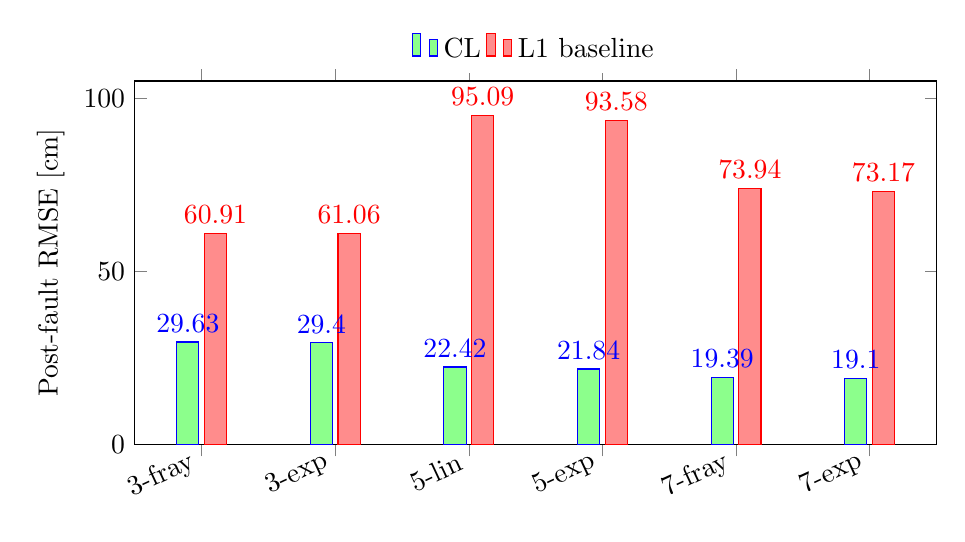
\begin{tikzpicture}
\begin{axis}[
  width=0.97\linewidth,
  height=6.2cm,
  ybar=2pt,
  bar width=8pt,
  ymin=0,
  ymax=105,
  ylabel={Post-fault RMSE [cm]},
  symbolic x coords={3-fray,3-exp,5-lin,5-exp,7-fray,7-exp},
  xtick=data,
  xticklabel style={rotate=25,anchor=east},
  legend style={at={(0.5,1.02)}, anchor=south, legend columns=2, draw=none},
  nodes near coords,
  nodes near coords align={vertical}
]
\addplot+[fill=green!45] coordinates {(3-fray,29.63) (3-exp,29.40) (5-lin,22.42) (5-exp,21.84) (7-fray,19.39) (7-exp,19.10)};
\addplot+[fill=red!45] coordinates {(3-fray,60.91) (3-exp,61.06) (5-lin,95.09) (5-exp,93.58) (7-fray,73.94) (7-exp,73.17)};
\legend{CL,L1 baseline}
\end{axis}
\end{tikzpicture}